%% abtex2-modelo-projeto-pesquisa.tex, v-1.7.1 laurocesar
%% Copyright 2012-2013 by abnTeX2 group at http://abntex2.googlecode.com/ 
%%
%% This work may be distributed and/or modified under the
%% conditions of the LaTeX Project Public License, either version 1.3
%% of this license or (at your option) any later version.
%% The latest version of this license is in
%%   http://www.latex-project.org/lppl.txt
%% and version 1.3 or later is part of all distributions of LaTeX
%% version 2005/12/01 or later.
%%
%% This work has the LPPL maintenance status `maintained'.
%% 
%% The Current Maintainer of this work is the abnTeX2 team, led
%% by Lauro César Araujo. Further information are available on 
%% http://abntex2.googlecode.com/
%%
%% This work consists of the files abntex2-modelo-projeto-pesquisa.tex
%% and abntex2-modelo-references.bib
%%

% ------------------------------------------------------------------------
% ------------------------------------------------------------------------
% abnTeX2: Modelo de Projeto de pesquisa em conformidade com 
% ABNT NBR 15287:2011 Informação e documentação - Projeto de pesquisa -
% Apresentação 
% ------------------------------------------------------------------------ 
% ------------------------------------------------------------------------

\documentclass[
	12pt,
	oneside,
	a4paper,
	english,
	brazil,
]{abntex2}

% ---
% PACOTES
% ---

% ---
% Pacotes fundamentais 
% ---
\usepackage{cmap}				% Mapear caracteres especiais no PDF
\usepackage{lmodern}			% Usa a fonte Latin Modern
\usepackage[T1]{fontenc}		% Selecao de codigos de fonte.
\usepackage[utf8]{inputenc}		% Codificacao do documento (conversão automática dos acentos)
\usepackage{indentfirst}		% Indenta o primeiro parágrafo de cada seção.
\usepackage{color}				% Controle das cores
\usepackage{graphicx}			% Inclusão de gráficos
\usepackage{xcolor}
% ---

% ---
% Pacotes de citações
% ---
\usepackage[brazilian,hyperpageref]{backref}	 % Paginas com as citações na bibl
\usepackage[alf]{abntex2cite}	% Citações padrão ABNT

% --- 
% CONFIGURAÇÕES DE PACOTES
% --- 

% ---
% Diretório das imagens
% ---
\graphicspath{ {Images/} }

% ---
% Configurações do pacote backref
% Usado sem a opção hyperpageref de backref
\renewcommand{\backrefpagesname}{Citado na(s) página(s):~}
% Texto padrão antes do número das páginas
\renewcommand{\backref}{}
% Define os textos da citação
\renewcommand*{\backrefalt}[4]{
	\ifcase #1 %
		Nenhuma citação no texto.%
	\or
		Citado na página #2.%
	\else
		Citado #1 vezes nas páginas #2.%
	\fi}%
% ---

% ---
% Informações de dados para CAPA e FOLHA DE ROSTO
% ---
\titulo{Aplicação de chamadas em sala de aula automatizado com Beacons}
\autor{Rafael Kellermann Streit}
\local{Brasil}
\data{2016}
\instituicao{%
  FACCAT - Faculdades Integradas de Taquara
  \par
  Graduação em Sistemas de Informação}
\tipotrabalho{Projeto de Pesquisa}
% O preambulo deve conter o tipo do trabalho, o objetivo, 
% o nome da instituição e a área de concentração 
\preambulo{Aplicação que faz as chamadas em sala de aula de maneira automatizada, utilizando Beacons.}
% ---

% ---
% Configurações de aparência do PDF final

% informações do PDF
\makeatletter
\hypersetup{
     	%pagebackref=true,
		pdftitle={\@title}, 
		pdfauthor={\@author},
    	pdfsubject={\imprimirpreambulo},
	    pdfcreator={LaTeX with abnTeX2},
		pdfkeywords={abnt}{latex}{abntex}{abntex2}{projeto de pesquisa}, 
		colorlinks=true,       		% false: boxed links; true: colored links
    	linkcolor=blue,          	% color of internal links
    	citecolor=blue,        		% color of links to bibliography
    	filecolor=magenta,      		% color of file links
		urlcolor=blue,
		bookmarksdepth=4
}
\makeatother
% --- 

% --- 
% Espaçamentos entre linhas e parágrafos 
% --- 

% O tamanho do parágrafo é dado por:
\setlength{\parindent}{1.3cm}

% Controle do espaçamento entre um parágrafo e outro:
\setlength{\parskip}{0.2cm}  % tente também \onelineskip

% ---
% compila o indice
% ---
\makeindex
% ---

% ----
% Início do documento
% ----
\begin{document}

% Retira espaço extra obsoleto entre as frases.
\frenchspacing 

% ----------------------------------------------------------
% ELEMENTOS PRÉ-TEXTUAIS
% ----------------------------------------------------------
% \pretextual

% ---
% Capa
% ---
\imprimircapa
% ---

% ---
% Folha de rosto
% ---
\imprimirfolhaderosto
% ---

% ---
% NOTA DA ABNT NBR 15287:2011, p. 4:
%  ``Se exigido pela entidade, apresentar os dados curriculares do autor em
%     folha ou página distinta após a folha de rosto.''
% ---

% ---
% inserir o sumario
% ---
\pdfbookmark[0]{\contentsname}{toc}
\tableofcontents*
% ---


% ----------------------------------------------------------
% ELEMENTOS TEXTUAIS
% ----------------------------------------------------------
\newpage
\textual

% ----------------------------------------------------------
% Introdução
% ----------------------------------------------------------
\chapter*[Introdução]{Introdução}
\addcontentsline{toc}{chapter}{Introdução}

O trabalho de pesquisa e desenvolvimento consiste na criação de uma aplicação capaz de substituir a marcação de presença atual em salas de aula, com o objetivo de ser mais assertiva, menos trabalhosa e mais rápida. A tecnologia utilizada para a identificação da presença do aluno chama-se \emph{Beacon} e está presente em praticamente todos os \emph{smartphones} atuais com suporte a \emph{Bluetooth 4.0}.

Além da marcação de presença dos alunos, a aplicação identifica pontos de interesse na instituição de ensino, informando aos gestores da instituição quais os locais mais frequentados pelos alunos e seus horários, informações que são adquiridas também através de \emph{Beacons}.

% ----------------------------------------------------------
% Problematização  
% ----------------------------------------------------------

\chapter{Problematização}

Atualmente, para que um professor de uma disciplina faça a marcação de presença dos alunos, é necessário algum tipo de interação entre o aluno e o professor. O que mais se utiliza é quando o professor faz a chamada em voz alta, um por um, e o aluno precisa responder, também em voz alta. Ou também, o aluno pode assinar uma ata em todas as aulas, marcando sua presença. Ambos os métodos tem diversos problemas:

\begin{itemize}
    \item Um enorme tempo de aula é gasto para a marcação de presença
    \item Um aluno poderia responder por outro na chamada, mesmo que o colega não esteja em aula, causando assim a presença de um aluno que não está em aula
    \item Pelo fato de o papel de chamada ser físico, muitas vezes acontece de o professor perder por algum motivo (furto, desastres naturais, acidentes, esquecimento, etc)
    \item Também pelo fato de ser manualmente preenchido, pode haver erro humano na marcação, dificultando o processo
\end{itemize}


% ----------------------------------------------------------
% Estado da arte  
% ----------------------------------------------------------

\chapter{Estado da arte}

\section{Instituição educacional}

\subscetion{Processo de chamada em sala de aula}

\section{Smartphones}

Em 2007, após o lançamento do iPhone, a popularização do termo \emph{smartphone} se tornou muito forte, mas o conceito é mais antigo do que isto \cite{smartphone-history-pictures}. Desde então, o número de \emph{smartphones} no mundo não parou de crescer, passando da marca de 2 bilhões em 2016, e o Brasil é o 6º País com maior número deles \cite{smartphone-numbers}.

\section{Beacons}

A tecnologia dos \emph{Beacons} começou a ficar mais popular por volta de 2013 \cite{beacon-what-is-it-forbes}, quando a Apple lançou ela junto ao novo iPhone, o modelo 5s. Junto com o lançamento da tecnologia no iPhone, a Apple colocou \emph{Beacons} em mais de 250 de suas lojas físicas \cite{beacon-apple-store-case}, trazendo assim uma experiência diferenciada para os clientes que entravam na loja, olhavam os produtos e faziam pedidos.

Muitas pessoas se confundem que o \emph{Beacon} pode ser considerado bastante similar a tecnologia \emph{RFID (Radio-Frequency Identification)}, porém seu uso se diferente em alguns aspectos importantes:

\begin{itemize}
    \item Utiliza \emph{Bluetooth} para se comunicar, tornando-se assim uma tecnologia mais fácil de ser utilizada, devido ao grande volume de dispositivos que já vem com a tecnologia. Estima-se que até 2018, cerca de 90\% dos dispositivos terão \emph{Bluetooth LTE (Low Energy)} \cite{beacon-devices-estimate-2018}
    \item Pelo fato de \emph{Beacons} serem mais robustos (em questões de hardware e firmware), eles se tornariam mais caros do que \emph{RFID} para uma linha de produção, por exemplo, onde a quantidade de tags utilizadas é imensa (uma por peça/produto). No sub-capítulo "Funcionamento" falarei mais sobre a complexidade do dispositivo e porque isto seria mais difícil.
    \item O \emph{Beacon} fornece maior privacidade e opções de segurança ao usuário, pois ele requer alguns passos e autorizações para seu funcionamento \cite{beacon-apple-store-case}.
\end{itemize}

\subsection{Componentes de um beacon}

Existem diversos modelos diferentes de \emph{Beacons}. Além das funcionalidades básicas, que explicarei a seguir, eles podem conter funcionalidades adicionais, como por exemplo: GPS, sensor de temperatura e conexão Wi-Fi \cite{beacon-sensors-easy-kontakt}.

Mas para o funcionamento básico de um \emph{Beacon}, é necessário que ele tenha apenas: uma bateria, um pequeno computador com um \emph{Bluetooth} e um \emph{firmware} que alimenta este computador, dizendo para o \emph{Beacon} o que deve ser feito e como ele deve se comportar, além de armazenar as informações do Beacon usados para sua identificação: \emph{UDID}, \emph{major} e \emph{minor}. Os sensores são opcionais para seu funcionamento básico \cite{beacon-basic-hardware}.

\begin{figure}[h]
\centering
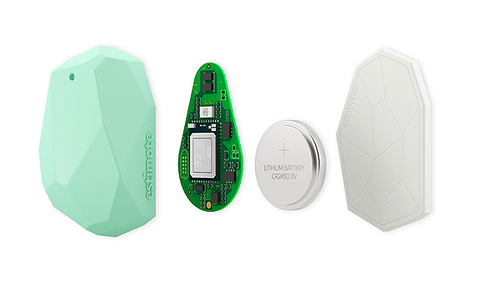
\includegraphics[width=0.7\textwidth]{estimote-beacon}
\caption{\emph{Beacon} da \emph{Estimote} com os componentes: capa de borracha (impermeável), \emph{hardware} com \emph{firmware} e \emph{Bluetooth}, bateria e protetor no fundo}
\end{figure}

\subsection{Funcionamento}

O funcionamento do Beacon, depende principalmente de três elementos que são configuráveis: o interval de disparo de sinal (normalmente em torno de 600ms) e a força do sinal, que é o que irá determinar a distância máxima atingida pelo Beacon. O sistema operacional \emph{iOS} faz o scan dos dispositivos a cada 1 segundo, isto significa que se o o Beacon estiver com intervalo de disparo em 330ms, o iOS irá receber três vezes o sinal naquele momento. Esta configuração normalmente é feita para lugares mais barulhentos, onde o sinal pode não chegar sempre ao celular, por motivos de outras ondas intereferirem na comunicação \cite{beacon-how-it-works-estimote}.

\subsection{Segurança}

O \emph{Beacon} é considerada uma tecnologia muito segura, principalmente pelo fato de ela depender da aprovação do usuário para seu funcionamento interferi-lo, pois em primeiro lugar, é necessário que o usuário tenha instalado um aplicativo que consiga ficar escutando as ondas de certos \emph{Beacons}, e mesmo que o usuário tenha o aplicativo instalado, ele ainda precisa aprovar o monitoramento dos \emph{Beacons}, podendo aprovar e restringir a qualquer momento \cite{beacon-what-is-it-forbes}.

\section{Tecnologias}
\subscetion{Swift}
\subscetion{Web Services}
\subsubsection{Infraestrutura}
\subsubsection{Django}
\subsubsection{JSON}


\chapter{Justificativa}

\chapter{Objetivos}
\section{Objetivos gerais}
\section{Objetivos específicos}

\chapter{Resultados esperados}

\chapter{Metodologia}
\section{Proposta do sistema}
\section{Desenvolvimento do sistema}
\subsection{Análise}
\subsection{Projeto}
\subsection{Codificação}
\subsection{Testes}
\subsection{Implantação}
\section{Tecnologias e ferramentas}



% ----------------------------------------------------------
% Orçamento  
% ----------------------------------------------------------

\chapter{Orçamento}

\begin{table}[ht]
\caption{Investimento Fixo}
\centering
\begin{tabular}{l c r r}
\hline\hline
Descrição & Quantidade & Valor unitário & Valor total \\ [0.5ex]
\hline
Apple MBPr 15" 16GB 500GB SSD&1&R\$18.000&R\$18.000 \\
iPhone 7 128GB&2&R\$4.000&R\$8.000 \\
Beacon Estimote&10&R\$120&R\$1.200 \\ [1ex]
\hline
\textbf{Total}&&&\textbf{R\$27.000} \\ [1ex]
\end{tabular}
\label{table:nonlin}
\end{table}

\begin{table}[ht]
\caption{Investimento Variável Mensal}
\centering
\begin{tabular}{l c r}
\hline\hline
Descrição & Quantidade &Valor \\ [0.5ex]
\hline
Servidor Ubuntu Server na AWS &1 (ou mais)&R\$100 \\
\hline
\textbf{Total}&&\textbf{R\$100} \\ [1ex]
\end{tabular}
\label{table:nonlin}
\end{table}


% ----------------------------------------------------------
% Cronograma  
% ----------------------------------------------------------

\chapter{Cronograma}

\begin{table}[ht]
\caption{Cronograma}
\centering
\begin{tabular}{lc}
    \hline
    Projeto de Pesquisa&2017 \\ [0.5ex]
    \hline
    \begin{tabular}{lcccccccccccc}
    Etapas do projeto& \cellcolor{blue!25} Jan&Fev&Mar&Abr&Mai&Jun&Jul&Ago&Set&Out&Nov&Dez \\
    Etapas do projeto&&&&&&&&&&&& \\
    Etapas do projeto&&&&&&&&&&&& \\
    \end{tabular}
\end{tabular}
\label{table:nonlin}
\end{table}


% ----------------------------------------------------------
% ELEMENTOS PÓS-TEXTUAIS
% ----------------------------------------------------------
\postextual

% ----------------------------------------------------------
% Referências bibliográficas
% ----------------------------------------------------------
\bibliography{Referencias}

% ----------------------------------------------------------
% Glossário
% ----------------------------------------------------------
%
% Consulte o manual da classe abntex2 para orientações sobre o glossário.
%
%\glossary

\end{document}
